\documentclass{article}
\usepackage{tikz}
\usetikzlibrary{positioning}

\begin{document}
\pagestyle{empty}

\def\layersep{2.7cm}

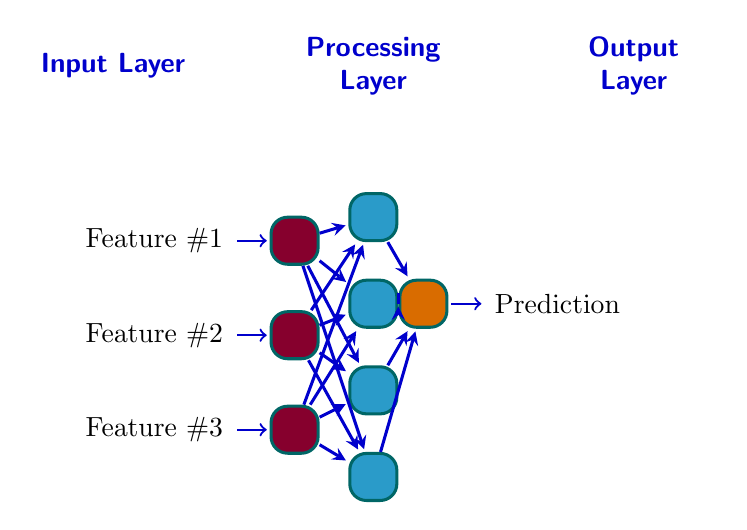
\begin{tikzpicture}[shorten >=1pt, -stealth, draw=blue!80!black, node distance=\layersep, line width=1.1pt]
    \tikzstyle{every pin edge}=[<-, shorten <=1pt, thick]
    \tikzstyle{unit}=[rectangle, rounded corners=6pt, fill=teal!60!black, minimum size=17pt, inner sep=0pt, draw=teal!80!black, line width=1.1pt]
    \tikzstyle{input unit}=[unit, fill=purple!70!black]
    \tikzstyle{output unit}=[unit, fill=orange!85!black]
    \tikzstyle{process unit}=[unit, fill=cyan!80!black]
    \tikzstyle{annot} = [text width=5.5em, text centered, font=\sffamily\bfseries, color=blue!80!black]

    % Draw the input layer nodes (renamed)
    \foreach \name / \y in {1,...,3}
        \node[input unit, pin=left:Feature \#\y] (I-\name) at (0,-\y*1.2) {};

    % Draw the processing layer nodes (renamed)
    \foreach \name / \y in {1,...,4}
        \path[yshift=0.2cm]
            node[process unit] (P-\name) at (\layersep,-\y*1.1 cm) {};

    % Draw the output layer node
    \node[output unit, pin={[pin edge={->, thick}]right:Prediction}, right=of P-2] (O) {};

    % Connect every node in the input layer with every node in the
    % processing layer.
    \foreach \source in {1,...,3}
        \foreach \dest in {1,...,4}
            \path (I-\source) edge (P-\dest);

    % Connect every node in the processing layer with the output layer
    \foreach \source in {1,...,4}
        \path (P-\source) edge (O);

    % Annotate the layers
    \node[annot, above=1.1cm of P-1] (pl) {Processing Layer};
    \node[annot, left=1.1cm of pl] {Input Layer};
    \node[annot, right=1.1cm of pl] {Output Layer};
\end{tikzpicture}
\end{document}